% Contextualização da prova (aparece apenas no caderno de questões)

\section*{Contextualização}

A aplicação \textbf{Copa Resultados} é um webapp que lista todas as partidas da
Copa do Mundo de 2026, da fase de grupos até a final. Os dados são obtidos do
projeto aberto \texttt{openfootball/worldcup.json} e armazenados no banco
\texttt{cupmatches}. A aplicação é composta por três partes:

\begin{itemize}
  \item \textbf{Backend (\texttt{api/})}: API em Node.js, TypeScript, Express e
        Mongoose, com os endpoints \texttt{GET /matches} (retorna o torneio com
        todas as partidas) e \texttt{GET /health} (verificação de saúde). Possui
        script de \emph{seed} que baixa o calendário oficial e popula o banco, e
        testes BDD com Cucumber.
  \item \textbf{Frontend (\texttt{web/})}: aplicação em Vite, TypeScript e React
        que consome a API e exibe as partidas. Em produção, os arquivos estáticos
        são servidos pelo Nginx.
  \item \textbf{Banco de dados}: MongoDB.
\end{itemize}

\begin{figure}[H]
  \centering
  % TODO: substituir o quadro abaixo pelo print do frontend
  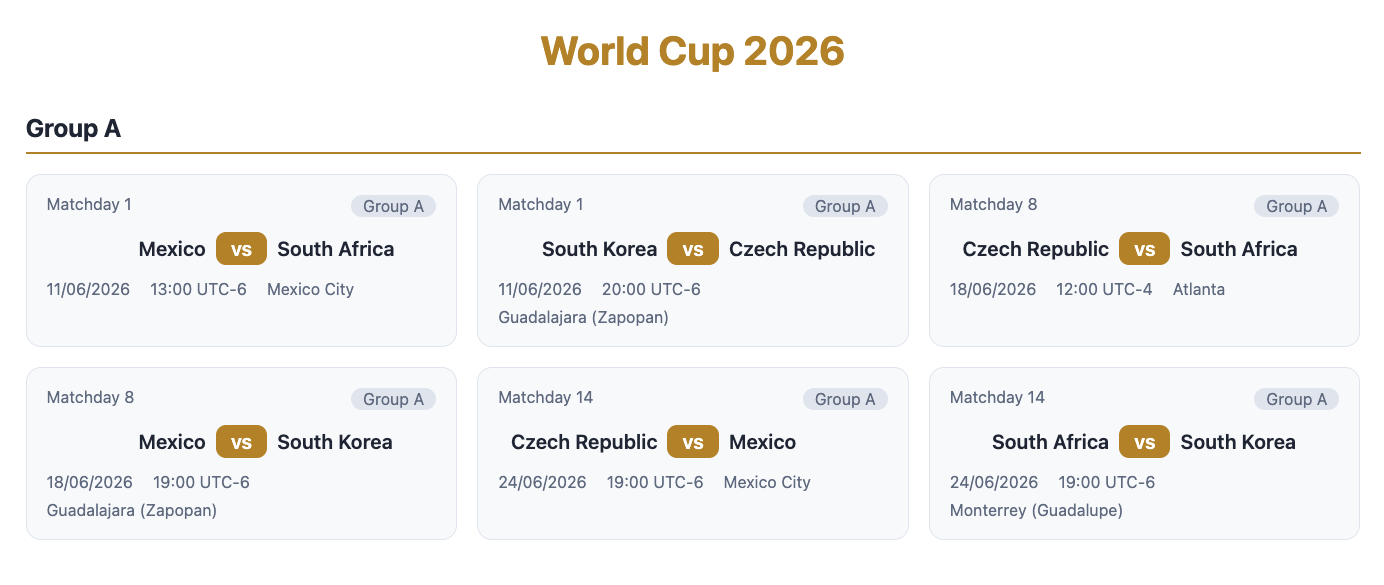
\includegraphics[width=0.9\textwidth]{cupmatches-screenshot.png}
%   \fbox{\parbox[c][6.5cm][c]{0.88\textwidth}{\centering \emph{Espaço reservado
%   para o print da tela principal do frontend}}}
  \caption{Tela principal do webapp Copa Resultados.}
\end{figure}

\subsection*{Estrutura do projeto}

O projeto está pronto e funcional, mas \textbf{ainda não está containerizado}.
A estrutura de pastas é a seguinte (os arquivos marcados são os que você deverá
escrever nesta prova):

\begin{lstlisting}
App/
|-- .github/
|   |-- workflows/
|       |-- api-test-bdd.yml  # <== QUESTAO 3
|-- api/                  # Backend (Node.js + TypeScript + Express + Mongoose)
|   |-- src/              # config/, controllers/, models/, routes/, seed.ts, server.ts
|   |-- features/         # Testes BDD (Cucumber)
|   |-- .env.dev          # Variaveis de ambiente (execucao local)
|   |-- Dockerfile        # <== QUESTAO 1
|-- web/                  # Frontend (Vite + React + TypeScript)
|   |-- src/              # components/, api.ts, App.tsx, main.tsx
|   |-- .env.dev          # Variaveis de ambiente (execucao local)
|   |-- nginx.conf        # Configuracao do Nginx (ja existe, pronta para uso)
|   |-- Dockerfile        # Ja existe, pronto para uso (nao e cobrado)
|-- docker-compose.yml    # <== QUESTAO 2
|-- .env                  # Variável de ambiente (lida automaticamente pelo Docker)
|-- README.md
\end{lstlisting}

\subsection*{Detalhes importantes do projeto}

\begingroup\sloppy
\begin{itemize}
  \item \textbf{Imagens}: Node 20 (\texttt{node:20-alpine}), Nginx
        (\texttt{nginx:alpine}) e MongoDB 7 (\texttt{mongo:7}).
  \item \textbf{Portas internas}: a API escuta na porta \texttt{3000}; o Nginx do
        container web escuta na porta \texttt{80}; o MongoDB usa a porta
        \texttt{27017}.
  \item \textbf{Rede do Docker Compose}: dentro da rede, a API acessa o banco pelo
        \textbf{nome do serviço} (\texttt{mongodb}), e não por \texttt{localhost}.
  \item \textbf{Build do frontend}: a variável \texttt{VITE\_API\_URL} é usada em
        \textbf{tempo de build} do Vite; por isso deve ser passada como
        \emph{build arg} para o Dockerfile do \texttt{web}.
  \item \textbf{Nginx}: o arquivo \texttt{web/nginx.conf} já existe e deve ser
        copiado para \texttt{/etc/nginx/conf.d/\allowbreak default.conf}; o build
        do Vite gera a pasta \texttt{dist}, que deve ser copiada para
        \texttt{/usr/share/\allowbreak nginx/\allowbreak html}.
  \item \textbf{Scripts npm do backend} (\texttt{api/package.json}):
\begin{itemize}
  \item \texttt{npm run dev} --- executa a API em modo de desenvolvimento, com
        recarga automática.
  \item \texttt{npm run build} --- compila o TypeScript para \texttt{dist/}.
  \item \texttt{npm start} --- executa a API já compilada (\texttt{node
        dist/server.js}).
  \item \texttt{npm run seed} --- baixa o calendário oficial e popula o banco.
  \item \texttt{npm run test:bdd} --- executa os testes BDD com Cucumber.
\end{itemize}
  \item \textbf{Variáveis de ambiente da raiz} (usadas pelo Docker Compose), com os
        valores exatos do projeto:

\begin{lstlisting}
API_PORT=3000
WEB_PORT=5173
MONGODB_PORT=27017
MONGODB_DATABASE=cupmatches
MONGODB_URI=mongodb://mongodb:27017/cupmatches
\end{lstlisting}

  \item \textbf{Execução local sem Docker}: os arquivos \texttt{api/.env.dev} e
        \texttt{web/.env.dev} já existem no projeto, com o seguinte conteúdo:

\begin{lstlisting}
# api/.env.dev
PORT=3000
MONGODB_URI=mongodb://localhost:27017/cupmatches

# web/.env.dev
VITE_API_URL=http://localhost:3000
\end{lstlisting}
  \item \textbf{Integração contínua}: o repositório deve possuir o workflow de
        \emph{GitHub Actions} \texttt{.github/\allowbreak workflows/\allowbreak
        api-test-bdd.yml}, que executa os testes BDD da API a cada \emph{push}
        no repositório remoto (detalhado na Questão 3).
  \item \textbf{Frontend já containerizado}: o arquivo \texttt{web/Dockerfile}
        já existe e está pronto para uso; nesta prova você não precisa escrevê-lo.
\end{itemize}
\endgroup
